% !TEX root = ../YourName-Dissertation.tex

\chapter{Neutrinos and Neutrino Masses}

\section{Introduction}



\section{Neutrinos}

The neutrino was first hypothesized by Dirac to explain the observation that beta-decay radiation is emitted in a continuous spectrum rather than a monoenergetic peak. Neutrinos, Italian for "little neutral one", were little more than a speculation when first hypothesize, so it is rather remarkable that neutrinos were eventually discovered by the work of Reines and Cowan in the 20th century. 

While first discovered in the context of nuclear physics, neutrinos have a pervasive presence throughout our universe. Not only are neutrinos important for our understanding of nuclear processes, but also to our understanding of cosmology and particle physics. It is fitting that the most abundant fermion in our universe should play a fundamental role in our understanding of the universe at is largest and smallest scales.

\section{Neutrino Oscillations}

Back in the day the solar neutrino problem was noticed in the experiment by Ray Davis. Neutrinos from the sun were missing. The experiment took place at the Sanford mine in South Dakota.

Neutrino oscillations were first observed by the Super-Kamiokande (SK) experiment in th 90's. The rates of atmospheric neutrinos from above and below were compared.

Neutrino oscillations were independently confirmed by the Sudbury Neutrino Observatory experiment (SNO) using solar neutrinos. 

Both experiments were awarded the Nobel prize in 2015 for the discover of neutrino oscillations.

Today the number of experiments which have measured rates of neutrino oscillation are legion. Measurements have been performed using various sources of neutrinos such as nuclear reactor, solar, atmospheric, and accelerator. 

The origin of neutrino oscillations is that the weak eigenstates are distinct from the mass eigenstates. The weakly interacting eigenstates are described as a superposition of the massive neutrino states using a 3x3 mixing matrix. 

The neutrino mixing matrix is typically written in the Pontecorvo-Maki-Nakagawa-Sakata (PMNS) parameterization.

\begin{figure}[htbp]
    \centering
    \includegraphics[width=0.6\textwidth]{figs/Chapter-2/230227_chap2_nu_hierarchy.png}
    \caption{Caption}
    \label{fig:chap2-nu-hierarchy}
\end{figure}

A giant experimental effort over the past couple of decades has greatly contained the majority of parameters in the PMNS matrix, many to relative uncertainties of only a few percent. However, some parameters still remain relatively unconstrained, which is the origin of the current uncertainty in the ordering of the neutrino masses. Next-generation neutrino oscillation experiments such as JUNO, Hyper-Kamiokande, and DUNE are poised to resolve this ambiguity in the coming years.

As one can see from the equation for neutrino mixing probabilities, the dependence on mass only enters as a difference between the mass eigenstates. Therefore oscillation probabilities are unaffected by the absolute scale of the neutrino mass. However, oscillations can be used to obtain a lower bound on the neutrino masses by setting the mass of the lightest neutrino mass state to zero. This results in different lower limits depending on the ordering of the neutrino mass states.

\begin{figure}[htbp]
    \centering
    \begin{subfigure}{0.7\textwidth}
        \includegraphics*[width=\textwidth]{figs/Chapter-2/230302_mass_estate_vals_normal.png}
        \caption{}
    \end{subfigure}
    \hfill
    \begin{subfigure}{0.7\textwidth}
        \includegraphics*[width=\textwidth]{figs/Chapter-2/230302_mass_estate_vals_inverted.png}
        \caption{}
    \end{subfigure}
    \caption{Caption}
    \label{fig:chap2-mass-estates}
\end{figure}

Various extensions to the 3x3 mixing regime, so called sterile neutrinos, have been proposed to explain certain anomalous neutrino oscillation phenomena observed primarily in neutrinos produced by nuclear reactors. Currently there is inconclusive evidence to support the existence of sterile neutrinos. Certain of these apparently anomalous results can be explained by better modeling of the nuclear processes in the reactors that generate the measured flux of neutrinos. However, some puzzles such as the unexplained neutrino deficits measured by the BEST experiment remain open.  

\section{Neutrino Masses in the Standard Model}

In modern quantum field theory spin-1/2 particles, or Fermions, are described using the Dirac equation. 

Fermion masses in the standard model are a result of the Higgs mechanism, which requires both left-chiral and right-chiral fermion fields. The current experimental evidence for neutrinos only support the existence of right-handed neutrinos and left-handed antineutrinos, therefore, neutrinos in the standard model are predicted to have zero mass. Consequently, the observation of neutrino oscillations is inconsistent with the standard model.

Since neutrinos are neutral particles, the simplest extension to the standard model is to allow neutrinos to have a Majorana mass term of the form \ldots If neutrinos are indeed Majorana fermions then one would predict that certain nuclei can decay via the rare neutrino-less double-beta decay process at a rate proportional to the neutrino mass absolute scale. 

Alternatively, if neutrinos are instead Dirac Fermions, one can generate neutrino masses in the standard model by allowing the existence of right-handed neutrino states. In this case neutrino masses are generated in the same way as other Fermions through the Yukawa coupling terms of the form \ldots These right-handed neutrino states are disallowed from interacting with the rest of the standard model other than gravitationally in order to be consistent with experimental data and are thus often referred to as "sterile neutrinos" due to their lack of weak interactions. Despite their lack of weak interactions it is possible for sterile neutrinos to be observed via their effects on neutrino oscillations.

These simple extensions to the standard model are dissatisfactory to many physicist, since they require coupling constants to the Majorana and Yukawa mass terms that are many orders of magnitude smaller than other fermions in order to generate neutrino masses consistent with observation data. The absolute masses of neutrinos are on the order of $10^{-6}$ smaller than the electron, which is suggestive that the origin of neutrino masses is the result of some new physics beyond the standard model.

A popular extension to the standard model to explain the smallness of the neutrino mass is the so-called see-saw mechanism \ldots

\section{Neutrino Absolute Mass Scale}

Neutrino oscillation probabilities are determined by the squared mass differences and are insensitive to the absolute neutrino mass scale, therefore, alternative probes are needed to perform an effective measurement of the neutrino mass.

\subsection{Limits from Cosmology}

In the $\Lambda$CDM model, which summarizes our current cosmological understanding of our universe, the mass-energy content of the universe is composed of approximately 27\% dark matter and only 5\% normal matter including neutrinos. From this observation, a rough limit on the neutrino mass can be obtained from the condition that neutrinos are not responsible for the entirety of the matter content of the universe. Using only this condition one can constrain the neutrino mass to be \ldots

A prediction of the $\Lambda$CDM model is that the universe originated from a single expansion event colloquially called the "Big Bang". In the Big Bang scenario, out universe originated as a hot spacetime singularity, which abruptly experience rapid expansion in a process called inflation. After the inflationary epoch the universe entered the reheating phase where the potential energy responsible for inflation decays into standard model particles such as electrons, quarks, and gluons. The universe continued to expand in size resulting in a decrease in energy density and lower temperature. Eventually the temperature of the universe decreased enough to allow the formation of protons, neutrons, and other baryons from quarks and gluons produced from the decays of the inflationary fields.

Also produced during the Big Bang are electrons, neutrinos and other leptons as well as a population of photons. These particles are kept in thermal equilibrium with the rest of the quark-gluon plasma through interactions that take place at the high temperatures and densities of the early universe. However, as the universe continues to expand it's density and temperatures decreases leading to the eventual decoupling of photons and leptons from the quarks and gluons. A prediction of inflation is that this population of photons produced during the Big Bang should still be present, but with a significantly reduced temperature due to the expansion of the universe. This is consistent with the observation of the CMB (cosmic microwave background), which is a population of microwave radiation with a blackbody temperature of 2.7~K. The CMB is extremely uniform in all directions with slight anisotropies that can be analyzed to study the evolution of the early universe. A series of experiments have measured the CMB with increasing levels of precision, which has lead to a significant increase in our current understanding of cosmology.

In addition to the CMB, inflation predicts the existence of a C$\nu$B (cosmic neutrino background), which are the remnant neutrinos produced during the Big Bang. Since neutrinos only interact via the weak force, they decouple from the hot Big Bang plasma at an earlier time than the CMB radiation. The temperature at which the C$\nu$B decouples depends on the neutrino rest mass. Neutrinos play a somewhat unique role in the $\Lambda$CDM model due to the fact that neutrinos act as radiation early in the universe but as matter in the late universe. This leads to unique signatures that impact anisotropies of the CMB as well as the distribution of matter in the universe. By combining measurements of the CMB with measurements of the large-scale structure (LSS) of the universe one can constrain the neutrino mass scale by fitting these datasets with the $\Lambda$CDM model. This analysis results in the some of the most stringent constraints on the neutrino mass. A recent analysis was able to constrain the neutrino mass scale to
\begin{equation}
     \Sigma_{m_\nu} \equiv \sum_{i}m_i<0.12~\mathrm{eV},
\end{equation}
where $m_i$ are the neutrino mass eigenstates. 

\begin{figure}[htbp]
    \centering
    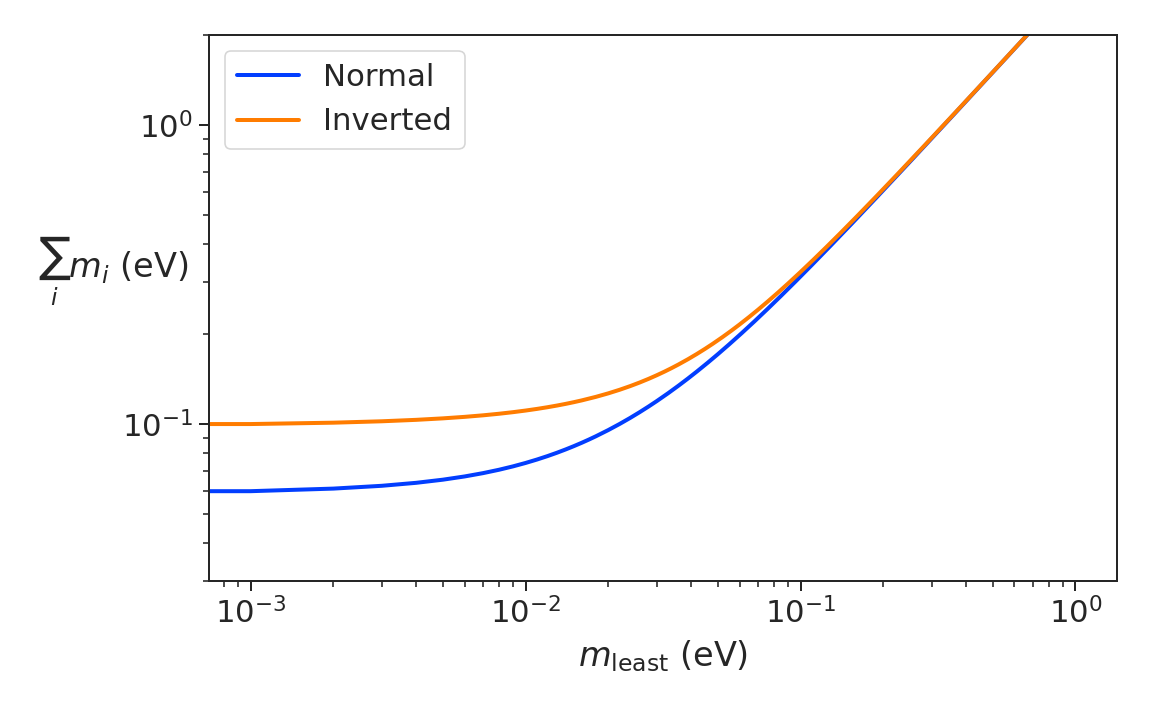
\includegraphics[width=0.7\textwidth]{figs/Chapter-2/230301_cosmology_nu_mass_observable.png}
    \caption{Caption}
    \label{fig:chap2-nu-mass-cosmo}
\end{figure}

The observable $\Sigma_{m_\nu}$ constrains the neutrino mass by setting the mass of the lightest neutrino mass eigenstate ($m_\mathrm{least}$). In the normal mass ordering $\Sigma_{m_\nu}$ can be rewritten in the form 
\begin{equation}
    \Sigma_{m_\nu} = m_\mathrm{least} + \sqrt{\Delta m_{21}^2+m_\mathrm{least}^2}+\sqrt{\Delta m_{32}^2+m_\mathrm{least}^2},
\end{equation}
where it is clear that a measurement of $\Sigma_{m_\nu}$ effectively sets the neutrino mass scale through $m_\mathrm{least}$. The analogous formula for the inverted mass ordering is 
\begin{equation}
    \Sigma_{m_\nu} = m_\mathrm{least}+\sqrt{-\Delta m_{32}^2+m_\mathrm{least}^2}+\sqrt{-\Delta m_{31}^2+m_\mathrm{least}^2}.
\end{equation}
In figure \ref{fig:chap2-nu-mass-cosmo} we plot the observable $\Sigma_{m_\nu}$ as a function of $m_\mathrm{least}$.

Upcoming experiments are planned to refine measurements of the CMB, LSS, and other cosmological observables. With this additional data it is possible that in the near future cosmological measurements will be able to positively constrain the neutrino absolute mass scale. However, the strength of these limits strictly depend on the accuracy of the $\Lambda$CDM model, which highlights the need for direct experimental measurements of the neutrino mass to confirm the predictions of cosmology and to fix the neutrino mass parameter in future cosmological analyses.

\subsection{Limits from Neutrinoless Double Beta-decay Searches}

If neutrinos are Majorana fermions then the neutrino is equivalent to its own antiparticle and lepton conservation is not an exact law of nature. Searches for lepton number violation, specifically the neutrinoless double beta-decay ($0\nu\beta\beta$) process, are some of the most powerful tests of lepton number conservation, which depend on the neutrinos being Majorana fermions. In double beta-decay two neutrons contained in the decay species nucleus spontaneously decay into two protons resulting in the production of two electrons and two neutrinos (see Figure \ref{fig:chap2-0nubetabeta-diagram}).  
\begin{figure}[htbp]
    \centering
    \begin{subfigure}{0.4\textwidth}
        \includegraphics*[width=\textwidth]{figs/Chapter-2/230717_2nubetabeta.png}
        \caption{}
    \end{subfigure}
    \begin{subfigure}{0.4\textwidth}
        \includegraphics*[width=\textwidth]{figs/Chapter-2/230717_0nubetabeta.png}
        \caption{}
    \end{subfigure}
    \caption{\label{fig:chap2-0nubetabeta-diagram} Feynman diagrams for double beta-decay (a) and $0\nu\beta\beta$(b).}
\end{figure}
However, for $0\nu\beta\beta$ the two neutrinos self-annihilate during the decay resulting only in the production of two electrons and a violation of lepton number by two. 

Assuming that the exchange of two Majorana neutrinos is the dominant channel for $0\nu\beta\beta$, then a measurement of the $0\nu\beta\beta$ half-life for a particular isotope can be used to set the neutrino absolute mass scale. The half-life is written in terms of the effective neutrino mass for $0\nu\beta\beta$ ($m_{\beta\beta}$) using the equation 
\begin{equation}
    T^{0\nu}_{1/2}=\frac{1}{G|\mathcal{M}|^2m_{\beta\beta}^2},
\end{equation}
where $G$ is the phase-space factor for the decay and $\mathcal{M}$ is the relevant nuclear matrix element. $m_{\beta\beta}$ is given by an incoherent sum of the neutrino mass eigenstates weighted by the PMNS mixing matrix parameters,
\begin{equation}
    m_{\beta\beta}=|\sum_{i}U_{ei}^2m_i|.
    \label{eq:chap2-mbetabeta}
\end{equation}

The information provided from $0\nu\beta\beta$ on the neutrino mass scale can be visualized by expressing the value of $m_{\beta\beta}$ in terms of $m_\textrm{least}$ and two relative Majorana phases. The allowed regions for $m_{\beta\beta}$ as a function of $m_\textrm{least}$ are shown in Figure \ref{fig:chap2-nu-mass-0nbb-posterior} as the regions bounded by the black curves overlayed with the discovery probabilities of future $0\nu\beta\beta$ decay experiments based on current neutrino data.
\begin{figure}[htbp]
    \centering
    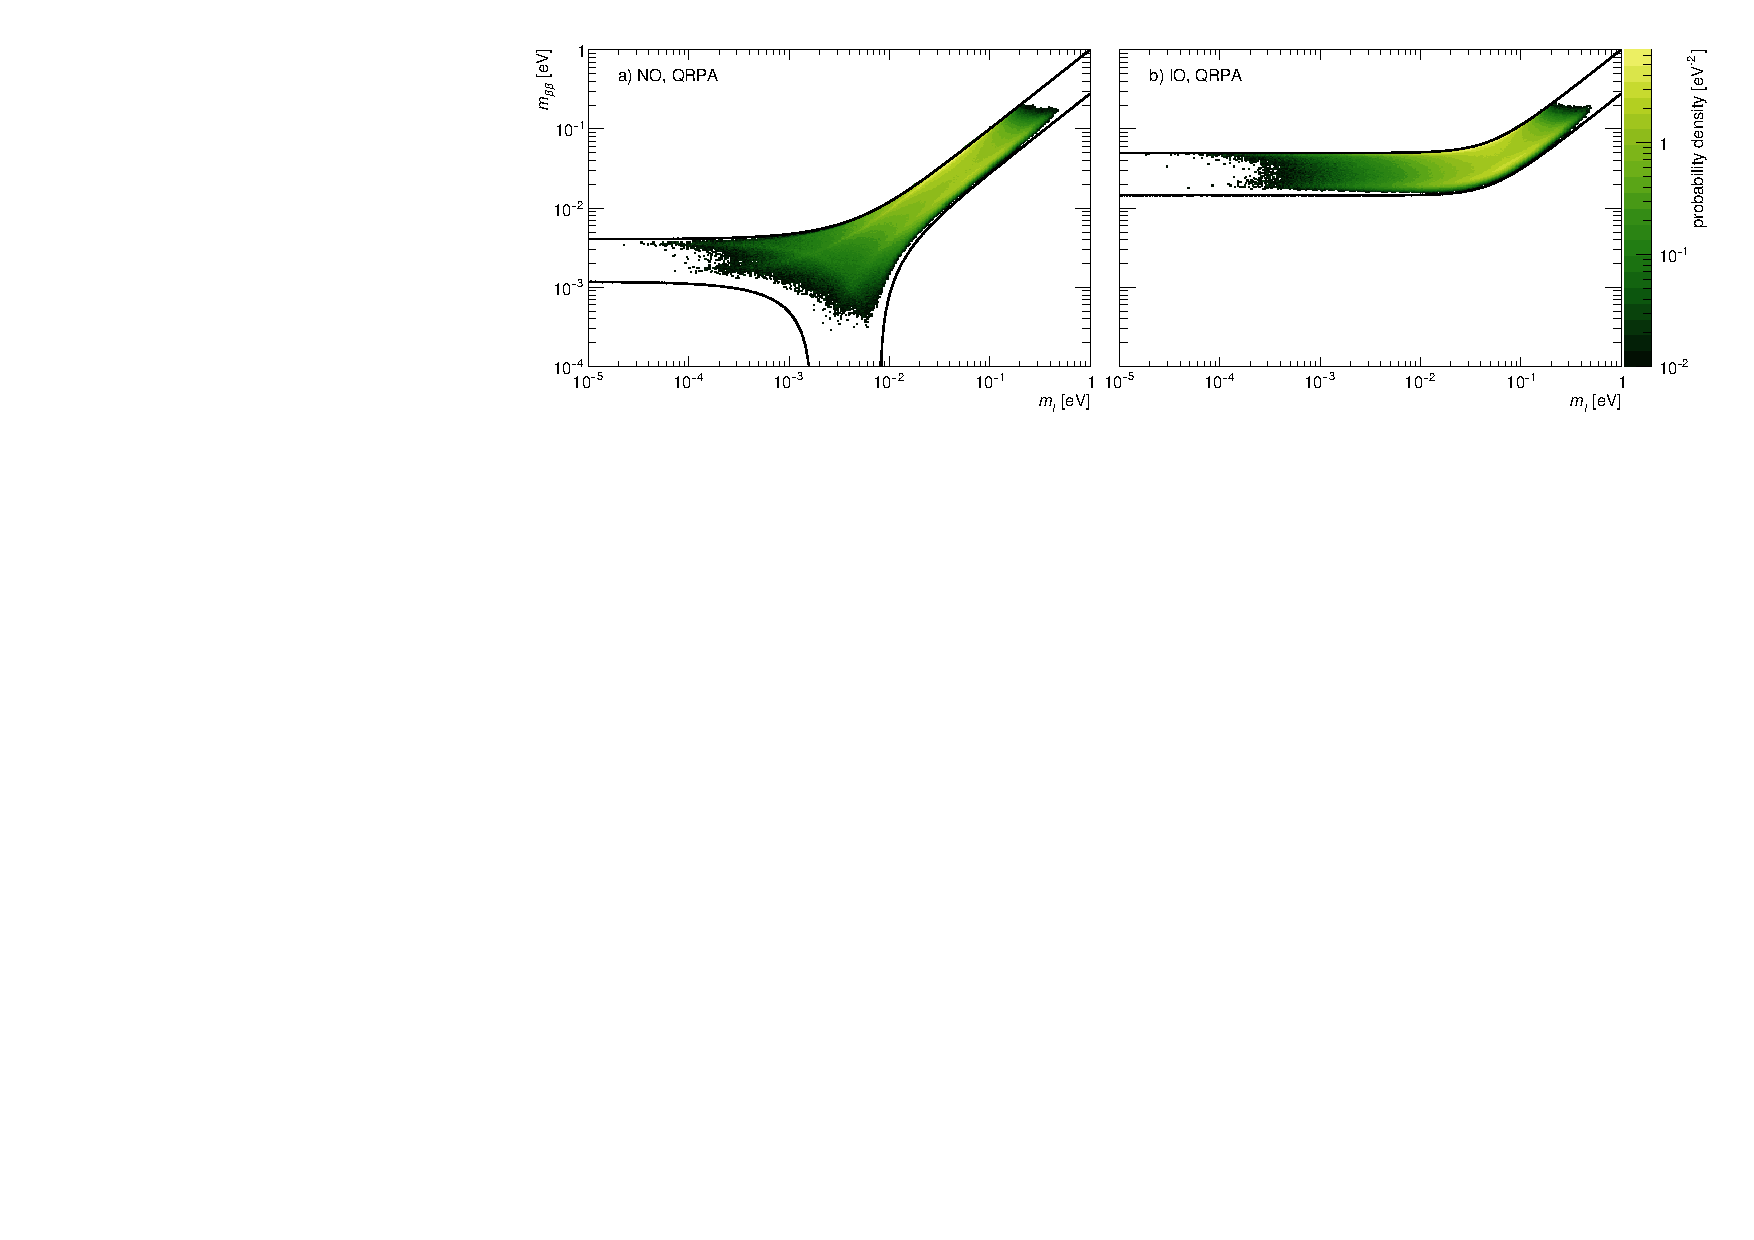
\includegraphics[width=1.0\textwidth]{figs/Chapter-2/230228_nu_mass_0nbb.pdf}
    \caption{The discovery probabilities for the future generation of $0\nu\beta\beta$ experiments as a function of $m_{\beta\beta}$ and $m_{least}$. }
    \label{fig:chap2-nu-mass-0nbb-posterior}
\end{figure}
Because of the possibility of cancellation due to the unknown Majorana phases included in the sum specified by Equation \ref{eq:chap2-mbetabeta}, the information gained is necessarily imperfect. Additionally, theoretical uncertainty in the calculation of the nuclear matrix elements complicates the calculation of $m_{\beta\beta}$ from a measurement of $0\nu\beta\beta$ half-life. Similar to cosmology there is a high degree of complementarity between direct measurements of the neutrino mass and $0\nu\beta\beta$. In particular, a measurement of $m_\textrm{least}$ to less than than 0.1~eV sensitivity provides significant information for $0\nu\beta\beta$ searches based of the discovery probabilities of Figure \ref{fig:chap2-nu-mass-0nbb-posterior}.

%\begin{figure}[htbp]
%    \centering
%    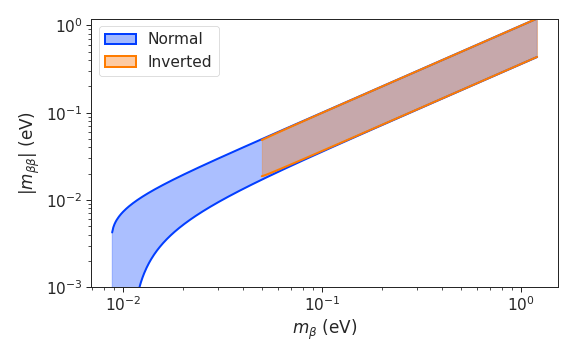
\includegraphics[width=0.7\textwidth]{figs/Chapter-2/230301_mbb_vs_mb.png}
%    \caption{Caption}
%    \label{fig:nu_mass_0nbb_vs_nu_beta}
%\end{figure}

\subsection{Limits from Beta-decay}

\begin{figure}[htbp]
    \centering
    \includegraphics*[width=0.6\textwidth]{figs/Chapter-2/230717_betadecay.png}
    \caption{\label{fig:chap2-beta-decay-diagram} A Feynman diagram of beta decay}
\end{figure}

Certain processes involving neutrinos, in particular beta-decay (see Figure \ref{fig:chap2-beta-decay-diagram}), have initial states with well-defined total energies and final states where the kinetic energies of each of the particles can be measured with high accuracy and precision. Beta-decay involves the decay of an unstable isotope where a neutron spontaneously converts to a proton and emits and electron and anti-neutrino ("neutrino" for brevity) to conserve charge and lepton number. Therefore, by applying the principles of energy and momentum conservation a measurement of the kinematics of the final state can be used to constrain the neutrino mass as proposed by Fermi in his 1934 description of nuclear beta-decay (see Figure \ref{fig:chap2-fermi-original-b-spectrum}).
\begin{figure}[htbp]
    \centering
    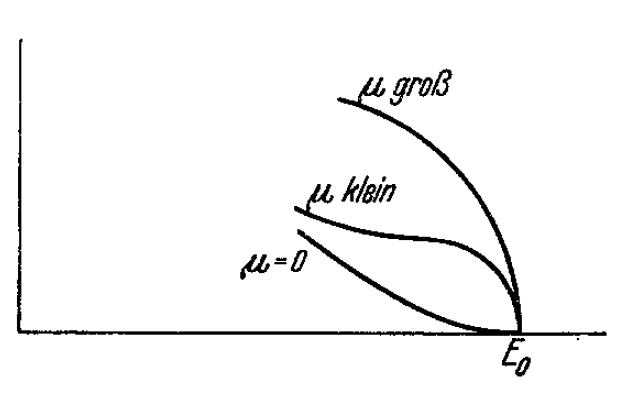
\includegraphics[width=0.5\textwidth]{figs/Chapter-2/Fermi.png}
    \caption{A figure from Fermi's 1934 paper on a theory of beta-decay depicting the kinetic energy spectrum of the emitted electron. The effect of the neutrino mass, written as $\mu$, is to distort the shape of the spectrum near the endpoint from the zero-mass spectrum.}
    \label{fig:chap2-fermi-original-b-spectrum}
\end{figure}
Because the constraint on the neutrino mass from beta-decay depends only on the final state measurement capabilities, such measurements of the neutrino mass are often referred to as model-independent or direct in contrast to constraints on the neutrino mass from cosmology and $0\nu\beta\beta$.

The beta-decay isotope of choice for direct neutrino mass measurements with beta-decay has been tritium ($^3H_2$) for many decades, because it conveniently fulfills many experimental requirements. Of upmost importance is a decay with a low Q-value, which is the available kinetic energy based on the mass difference between the initial and final states. The effect of a massive neutrino on the shape of the spectrum is magnified for low Q-values and tritium decays have an unusually low Q-value of 18.6~keV. Additionally, tritium beta-decay is a super-allowed decay, which means that is has a relatively short half-life of 12.3~years making it easy to obtain a high-activity source with a relatively small source mass. High-activity is desireable due to the low-activity near the tritium spectrum endpoint. For tritium beta-decays only a factor of $3\times10^{-13}$ of the decays occur in the last 1~eV of the spectrum. Isotopes with Q-values lower than tritium are known, but this is outweighed by exceedingly long half-lives leading to unobtainable source masses.

Neutrino mass measurements using beta-decay measure the effect of the neutrino's mass on shape of the electron's kinetic energy spectrum near the endpoint. The kinetic energy spectrum (see Figure \ref{fig:chap2-tritium-spectrum})is given by 
\begin{equation}
\begin{split}
    \frac{d\Gamma}{dE}=&\frac{G_F^2|V_{ud}|^2}{2\pi^3}(G_V^2+3G_A^2)F(Z,\beta)\beta(E+m_e)^2(E_0-E)\\
    &\times \sum_{i=1,2,3}{|U_{ei}|^2[(E_0-E)^2-m_i^2]^{1/2}\Theta(E_0-E-m_i)},
\end{split}
\end{equation}
\begin{figure}[htbp]
    \centering
    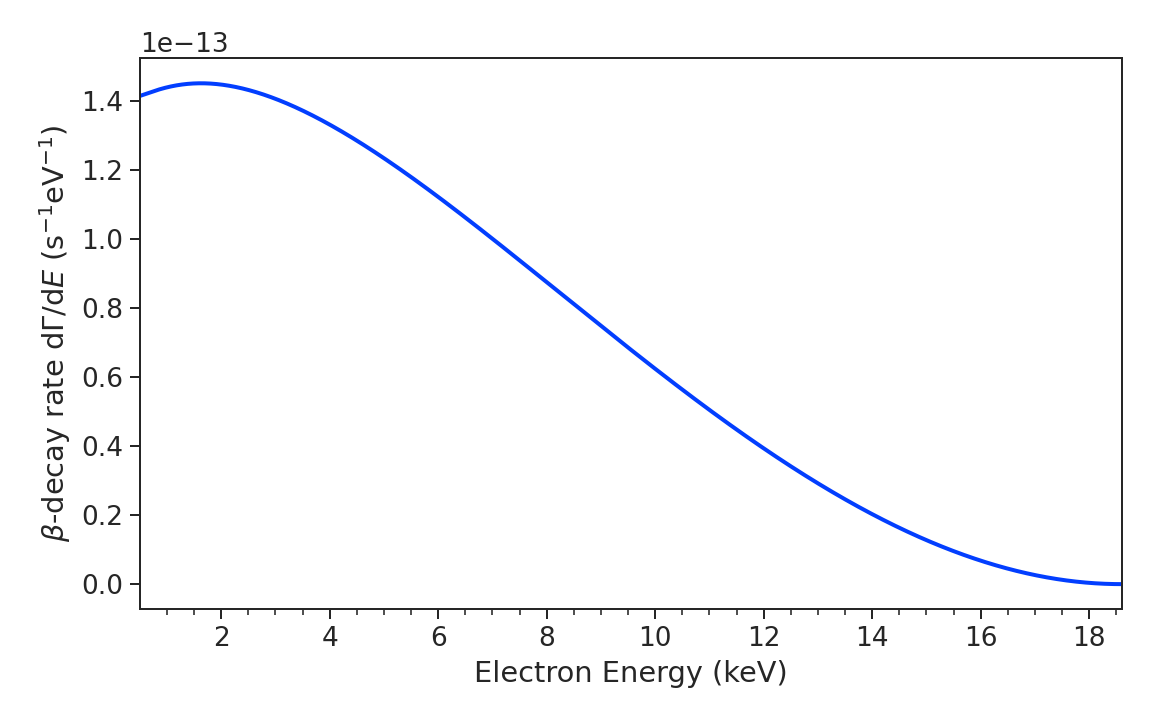
\includegraphics[width=0.7\textwidth]{figs/Chapter-2/230302_atomic_tritium_spectrum.png}
    \caption{Caption}
    \label{fig:chap2-tritium-spectrum}
\end{figure}
where $G_F$ is the Fermi coupling constant, $V_{ud}$ is an element of the CKM matrix, $E$ is the kinetic energy of the electron, $\beta$ is the velocity of the electron divided by the speed of light, $E_0$ is the endpoint energy assuming zero neutrino mass, $F(Z,\beta)$ is the Fermi function, and $\Theta(E_0-E-m_i)$ is the Heviside function, which enforces energy conservation. One can see that the decay spectrum is actually a combination of three spectra with different endpoints based on the actual values of the neutrino mass eigenstates, $m_i$. This results in "kinks" in the spectrum shape due to the overlapping spectra but such an effect would be nearly impossible to resolve given the finite energy resolution of a real experiment. 

The neutrino mass scale variable measured by beta-decay is given by 
\begin{equation}
    m_\beta^2=\sum_i{|U_{ei}|^2}m_i^2,
\end{equation}
where $m_beta$ is the effective mass of the neutrino in beta-decay or simply neutrino mass for brevity. By assuming unitarity, the neutrino mass can be expressed in terms of the PMNS matrix elements, squared mass differences, and the lightest neutrino mass eigenstate. For the normal mass ordering the equation is
\begin{equation}
    m_\beta^2=m^2_\textrm{least} + |U_{e2}|^2\Delta m_{21}^2 +|U_{e3}|^2\Delta m_{31}^2,
\end{equation} 
and for the inverted ordering the equation is 
\begin{equation}
    m_\beta^2=m^2_\textrm{least}+|U_{e1}|^2(-\Delta m_{32}^2-\Delta m_{21}^2)+|U_{e2}|^2(-\Delta m_{32}^2).
\end{equation}
Therefore, a measurement of the neutrino mass in combination with neutrino mixing parameters is effectively a measurement of $m_\textrm{least}$.

Since the neutrino mass is small ($<1$~eV), it's effect on the spectrum is limited to the endpoint region.
\begin{figure}[htbp]
    \centering
    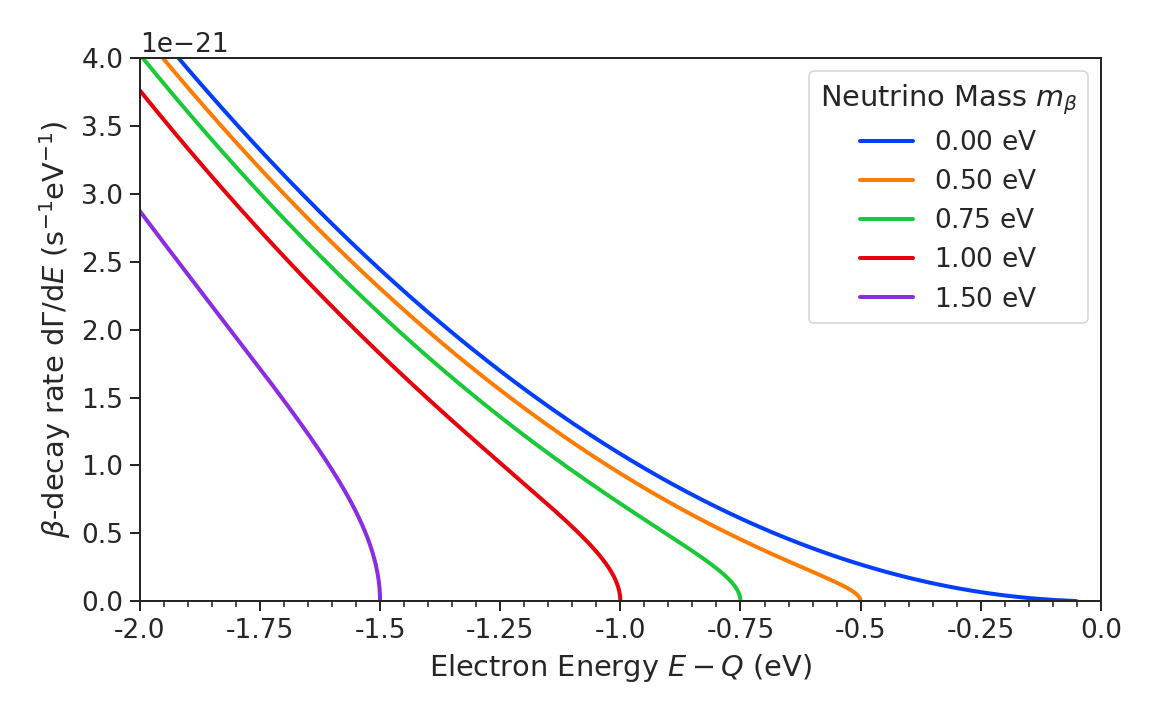
\includegraphics[width=0.7\textwidth]{figs/Chapter-2/230302_atomic_tritium_spectrum_near_endpoint.png}
    \caption{Caption}
    \label{fig:chap2-atomic-tritium-endpoint}
\end{figure}
The affect of a non-zero neutrino mass on the endpoint spectrum is plotted for the reader in Figure \ref{fig:chap2-atomic-tritium-endpoint}. Resolving the small changes in the spectrum shape requires an experimental technique with high statistics,, excellent energy resolution, as well as low background activity. The KATRIN collaboration 